\documentclass[12pt,oneside,openany,pagenumber=footcenter]{book}
%\documentclass[a4paper,10pt]{report}

\usepackage[utf8]{inputenc}
\usepackage{lmodern}
\usepackage[T1]{fontenc}
\usepackage{amsfonts}
\usepackage{amsmath,amsthm}
\usepackage{import}

\usepackage{fontenc}
\usepackage{graphicx}
\usepackage{graphics}
\usepackage{graphicx}
\usepackage{hyperref}
\usepackage{makeidx}

\newtheorem{definition}{Definition}[section]
\newtheorem{HLPpoznamka}{Note}[section]
\newtheorem{HLPpriklad}{Example}[section]
\newtheorem{HLPcvicenie}[HLPpriklad]{Exercise}
\newtheorem{HLPdokaz}{Proof}[section]
\newtheorem{zadanie}{Task}[section]
\newenvironment{poznamka}{\begin{HLPpoznamka}\rm}{\end{HLPpoznamka}}
\newenvironment{example}{\begin{HLPpriklad}\rm}{\end{HLPpriklad}}
\newenvironment{cvicenie}{\begin{HLPcvicenie}\rm}{\end{HLPcvicenie}}
\newenvironment{dokaz}{\begin{HLPdokaz}\rm}{\end{HLPdokaz}}
\newtheorem{veta}{Theorem}[section]
\newtheorem{lemma}[veta]{Lemma}
\newtheorem{dosledok}[veta]{Corollary}
\newtheorem{teza}[veta]{Proposition}


\pagestyle{headings}

\bibliographystyle{../lib/eptcs}

\def\indexname{Register}
% pekne pokope definujeme potrebne udaje
\def\mftitlea{Biologically inspired computation models}
\def\mftitle{\mftitlea}
\def\mfthesistype{Dissertation thesis}
\def\mfauthor{Mgr. Michal Kováč}
\def\mfadvisor{doc. RNDr. Damas Gruska, PhD.}
\def\mfplacedate{Bratislava, 2015}


\ifx\pdfoutput\undefined\relax\else\pdfinfo{ /Title (\mftitle) /Author (\mfauthor) /Creator (PDFLaTeX) } \fi

\def\eps{\varepsilon}
\def\goodgap{\hspace{\subfigcapskip}}
\makeindex

\begin{document}
\frontmatter
\thispagestyle{empty}
\begin{minipage}{0.20\textwidth}

\includegraphics[width=0.9\textwidth]{img/comenius_half.png}
\end{minipage}
\begin{minipage}{0.79\textwidth}
\begin{center}
\sc Department of Applied Informatics \\
Faculty of Mathematics, Physics and Informatics \\
Comenius University, Bratislava
\end{center}
\end{minipage}

\vfill
\begin{center}
\begin{minipage}{0.8\textwidth}
\hrule
\bigskip\bigskip
\centerline{\LARGE\sc\mftitlea}
\smallskip
\centerline{(\mfthesistype)}
\bigskip
\bigskip
\centerline{\large\sc\mfauthor}
\bigskip\bigskip
\hrule
\end{minipage}
\end{center}
\vfill
{\bf Advisor:} \mfadvisor
\hfill\mfplacedate
\eject
\eject

\thispagestyle{empty}
{~}\vspace{12cm}

{~}\vspace{12cm}

\begin{minipage}{0.25\textwidth}~\end{minipage}
\begin{minipage}{0.69\textwidth}
I hereby declare that this submission is my own work and that, to the best of my knowledge and belief, it contains no material previously published or written by another person nor material which to a substantial extent has been accepted for the award of any other degree or diploma of the university or other institute of higher learning, except where due acknowledgment has been made in the text.

\bigskip\bigskip

\hfill\hbox to 6cm{\dotfill}
\end{minipage}

\chapter*{Acknowledgements}

I am very grateful to all the people I had the privilege to work with, especially I would like to thank my advisor RNDr. Damas Gruska PhD. for his constant interest, encouragement and help that I deeply appreciate.
The present work was possible due to many beneficial consultations and intensive cooperation.

I would also like to thank to the members of Laboratory of Comparative and Functional Genomics of Eukaryotic Organelles and their head, Prof. Ľubomír Tomáška for familiarization with the work of biologists.

I thank to my family, colleagues, teammates and all the friends who supported me especially last weeks before the deadlines for their patience, support and understanding\footnote{Understanding that they will propably never understand my work;)}

% Osobitná vďaka patrí vedúcemu diplomovej práce doc. RNDr. Damasovi Gruskovi PhD. za cenné rady, námety, podnetné pripomienky a všestrannú pomoc, ktorú si hlboko vážim. Len vďaka mnohým prínosným konzultáciam a intenzívnej spolupráci som bol schopný napísať toto dielo. Nesmiem zabudnúť ani na RNDr. Branislava Rovana, CSc. a spolužiakov za to, že si na dizertačnom seminári našli čas, aby si vypočuli moju prezentáciu dizertačnej práce. Ďalšie poďakovania venujem rodičom a známym, ktorí to so mnou dokázali vydržať posledné týždne pred odovzdaním.

% !TEX root = diz.tex
\chapter*{Abstract}
\begin{description} \itemsep1pt \parskip0pt \parsep0pt
  \item[Author:] \mfauthor
  \item[Title:] \mftitle
  \item[University:] Comenius University in Bratislava
  \item[Faculty:] Faculty of Mathematics, Physics and Informatics
  \item[Department:] Department of Applied Informatics
  \item[Supervisor:] \mfadvisor
\end{description}

This work discusses the research in the membrane systems, an emerging field of natural computing. Many variants of membranes systems have already been studied, most of them uses parallel rewriting and are computationally complete. Various sequential models have been proposed, however, in many cases they are weaker than their parallel variant.

We propose some other sequential models, provide universality proofs for them and suggest further research.

\begin{description}
  \item[Keywords:] Computation models inspired by biology, Membrane systems, P systems
\end{description}

\chapter*{Abstrakt}
\begin{description} \itemsep1pt \parskip0pt \parsep0pt
  \item[Autor:] \mfauthor
  \item[Názov dizertačnej práce:] \mftitle
  \item[Škola:] Univerzita Komenského v Bratislave
  \item[Fakulta:] Fakulta matematiky, fyziky a informatiky
  \item[Katedra:] Katedra aplikovanej informatiky
  \item[Vedúci dizertačnej práce:] \mfadvisor
  \item \mfplacedate
\end{description}

V tejto práci sa zaoberáme výskumom v oblasti membránových systémov. Veľa variantov už bolo preskúmaných, väčšinou pri výpočte používajú paralelizmus a sú Turingovsky úplné. Navrhlo sa aj veľa sekvenčných modelov, ale väčšina z nich má slabšiu výpočtovú silu ako ich paralelný variant.

V druhej časti predkladáme niektoré sekvenčné modely, u ktorých dokazujeme Turingovu úplnosť a navrhujeme modely, ktoré plánujeme preskúmať v rámci dizertačnej práce.

\begin{description}
  \item[Kľúčové slová:] Výpočtové modely inšpirované biológiou, Membránové systémy, P systémy
\end{description}
\tableofcontents{}
\listoffigures{}
% \listoftables{}

\mainmatter

\chapter*{Introduction} % (fold)
\label{cha:introduction}
% !TEX root = diz.tex
\addcontentsline{toc}{chapter}{Introduction}

There are a lot of areas in the theoretical computer science that are motivated by other science fields. Computation models motivated by biology forms a large group of them. They include neural networks, computational models based on DNA evolutionary algorithms, which have already found their use in computer science and proved that it is worth to be inspired by biology. L-systems are specialized for describing the growth of plants, but they have also found the applications in computer graphics, especially in fractal geometry. Other emerging areas are still awaiting for their more significant uses.

One of them is the membrane computing \cite{Paun10OxfordHandbookMembraneComputing}. It is relatively young field of natural computing - in comparison: neural networks have been researched since 1943 and membrane systems since 1998 \cite{Paun98}.

Membrane systems (P systems) are distributed parallel computing devices inspired by the structure and functionality of cells. Recently, many P system variants have been developed in order to simulate the cells more realistically or just to improve the computational power.

We will start by an introduction of some natural computing areas including models inspired by biology in Chapter \ref{cha:natural_computing}. In Chapter \ref{cha:preliminaries} we recall some computer science basic notions that we will use through the work. P systems are formally presented in Chapter \ref{cha:p_systems}, with the current state of the research in their variants, overview of software simulator MeCoSym and various case studies.

In Chapter \ref{cha:on_the_edge_of_universality_of_sequential_p_systems} we will present the current state of our work, mainly from theoretic viewpoint (computational power, decidability of behavioral properties), including the published results in sections \ref{sec:inhibitors}, \ref{sec:active_membranes} and \ref{sec:notions_from_reaction_systems}.


% chapter introduction (end)

\chapter{Natural computing} % (fold)
\label{cha:natural_computing}
% !TEX root = diz.tex
Recently, an interdisciplinary research between the fields of Computer Science and Biology has been rapidly growing. Natural computing consists of three classes of methods:
\begin{itemize}
  \item those that are based on the use of computers to simulate natural phenomena
  \item those that employ natural materials (e.g., molecules) to compute
  \item those that take inspiration from nature for the development of novel problem-solving techniques
\end{itemize}

% Bioinformatics (slaves of biologists)

\section{Bioinformatics} % (fold)
\label{sec:bioinformatics}

Bioinformatics has undergone a fast evolving process, especially the areas of genomics and proteomics. Bioinformatics can be seen as the application of computing tools and techniques for the management of biological data. Just to mention a few:
\begin{itemize} 
  \item the design of efficient algorithms for DNA sequence alignment,
  \item the investigation of methods for prediction of the three-dimensional structure of molecules and proteins,
  \item the development of data structures to effectively store huge amount of structured data.
\end{itemize}

% section bioinformatics (end)

\section{Biomolecular computing} % (fold)
\label{sec:biomolecular_computing}

Biomolecular computing make use of molecules such as DNA and proteins to perform computations involving storing, retrieving and processing data. It takes advantage of the many different molecules to try many different possibilities at one, so it is somewhat similar to parallel computing.

Adleman in his 1994 report \cite{Adleman1994MolecularComputation} demonstrated a proof of concept use of DNA as a form of computation which solved the Hamiltonian path problem. Since then, various Turing machines have been proven to be constructible with DNA \cite{Kari2000DNAPCP}. 

DNA can also be used as a digital data storage with 5.5 petabits per cubic millimeter of DNA (see \cite{Church2012DNAStorage}). The information retrieval is, however, a slow process, as the DNA needs to be sequenced in order to retrieve data, so this method is intended mainly for a long-term archival of large amounts of scientific data.

% section biomolecular_computing (end)

\section{Biologically inspired computing models} % (fold)
\label{sec:biologically_inspired_computing_models}

On the other hand, the birth of biologically inspired frameworks started the investigation of mathematical models and their properties and technological requirements for their implementation by biological hardware.
Those frameworks are inspired by the nature in the way it ``computes'', and has gone through the evolution for billions of years.

Neural networks, genetic algorithms and DNA computing are already well established research fields.

\subsection{Neural networks} % (fold)
\label{sub:neural_networks}

Inspired by the human brain, which contains on average 86 billions neurons \cite{Azevedo09NumberOfNeurons}, neurophysiologist Warren McCulloch in 1943 proposed a mathematical model of artificial \index{Neural network} neural network.

A single perceptron computes a function $f(x)$, where $x$ is an input - a vector of real values.

The perceptron can learn itself by modifying parameters used to compute the function. This learning can be performed in various ways, we will mention only the supervised learning. Imagine a function with
\begin{itemize}
  \item input: perceptron's parameters
  \item output: error of the computed result $f(x)$
\end{itemize}
If the perceptron receives a feedback in form of error (from the supervision, e.g. dataset used to train the perceptron), it can modify its parameters such the error will be minimized in the future. This can be done through the gradient descent method, which is used to find a local minimum of a function.

A single perceptron can only compute linear functions, so they are often connected with other perceptron to form a neural network. Often it is practically unusable to say what is the purpose of a single neuron in a more complex neural networks.

Neural networks have broad applicability to real world problems and are best if the modeled system has some tolerance to error such as:
\begin{itemize}
  \item Image recognition: OCR, web search by image
  \item Music recognition by voice sample
  \item Speech recognition
  \item Time series forecast: weather, stock
  \item Diagnosing of illnesses
  \item Natural language processing
\end{itemize}

Besides real world problems, Graves et al. \cite{Graves14NeuralTM} extended the capabilities of neural networks by coupling them to external memory resources, allowing them to infer simple algorithms such as copying and sorting.

% subsection neural_networks (end)

\subsection{Evolutionary algorithms} % (fold)
\label{sub:evolutionary_algorithms}

\index{Evolutionary algorithms} Evolutionary algorithms are inspired by Darwin's theory of evolution. Basically, an algorithm starts with a population of random individuals (solutions to the problem). In each generation, the fitness of every individual is evaluated and the more fit individuals are replicated and mutated to form a new generation. The less fit individuals die.

Idea of evolutionary computing was introduced in the 1960's by I. Rechenberg. Nowadays they have been applied to find solution of many optimization problems. They also can be used to design or to train a neural network \cite{Montana:1989:TrainNeuronByGenetic}.

% subsection evolutionary_algorithms (end)

\subsection{L systems} % (fold)
\label{sub:l_systems}

In 1968, a Hungarian botanist and theoretical biologist Aristid Lindenmayer introduced a new string rewriting algorithm named Lindenmayer systems (or \index{L-systems} L-systems for short) \cite{Lindenmayer68, Rozenberg12Lindenmayer}. Inspired by the growth of plants, they have proven to be among the most beautiful examples of interdisciplinary science, where work in one area induces fruitful ideas and results in other areas:
\begin{itemize}
  \item Computer graphics - simulated evolution of plants, where L-systems are used as genetic encoding. The phenotypes are the branching structures resulting from the derivation and graphic interpretation of the genotypes \cite{Ochoa98GeneticLSystems}.
  \item Abstract framework for music composers to allow generation of musical structure \cite{Manousakis06MusicalLSystems}.
  \item Generating nonlinear missions in PC games, where multiple possible paths can lead to the goal of the mission \cite{Togelius2016LSystemsLevels}.
\end{itemize}

% subsection l_systems (end)

\subsection{Swarm Intelligence} % (fold)
\label{sub:swarm_intelligence}

Swarm intelligence \index{Swarm intelligence} systems conists of a population of simple agents, which are following simple rules. They coordinate in decentralized manner and self-organize to achieve a common goal. The swarm intelligence focuses on the collective behaviors that result from the local interactions of the individuals with each other and with their environment. Examples of such systems are colonies of ants and termites, schools of fish, flocks of birds, herds of land animals and bees.

The solutions designed by nature can often be used in other real-world problems.

\subsubsection{Ant colony optimization} % (fold)
\label{ssub:ant_colony_optimization}

Ant colony optimization \index{Ant colony optimization} introduced by Dorigo \cite{Dorigo96Ants} is a class of optimization algorithms for finding better paths through graphs. Ants wander randomly to find some food and return to their colony while laying down pheromone trails. If other ants find such a path, they are likely not to keep travelling at random, but instead to follow the trail, returning and reinforcing it if they eventually find food. Over time, however, the pheromone trail starts to evaporate, thus reducing its attractive strength. The more time it takes for an ant to travel down the path and back again, the more time the pheromones have to evaporate. A short path, by comparison, gets marched over more frequently, and thus the pheromone density becomes higher on shorter paths than longer ones. Pheromone evaporation also has the advantage of avoiding the convergence to a locally optimal solution. If there were no evaporation at all, the paths chosen by the first ants would tend to be excessively attractive to the following ones. In that case, the exploration of the solution space would be constrained. The influence of pheromone evaporation in real ant systems is unclear, but it is very important in artificial systems \cite{Dorigo04Ants}. It has been used to produce near-optimal solutions to the travelling salesman problem. They have an advantage over simulated annealing and genetic algorithm approaches of similar problems when the graph may change dynamically, the ant colony algorithm can be run continuously and adapt to changes in real time. Among other real-world uses are the vehicle routing problem \cite{Rizzoli07AntsVehicle} and improving the efficiency of an electric motor in dry vacuum cleaner \cite{Korosec09AntsVacuum}.

% subsubsection ant_colony_optimization (end)

\subsubsection{Bird flocking} % (fold)
\label{ssub:bird_flocking}

In the natural world, organisms exhibit certain behaviors when traveling in groups. This phenomenon, also known as flocking\index{flocking}, occurs at both microscopic scales (bacteria) and macroscopic scales (birds, fish, insects). Using computers, these patterns can be simulated by creating simple rules for interaction with neighbors and combining them to a complex collective behavior:
\begin{itemize}
  \item Alignment is a behavior that causes a particular agent to line up with agents close by.
  \item Cohesion is a behavior that causes agents to steer towards the center of mass of neighbors - that is, the average position of the agents within a certain radius.
  \item Separation is the behavior that causes an agent to steer away from all of its neighbors to avoid clashes.
\end{itemize}
Reynolds in 1987 first used such rules in a simulation \cite{Reynolds87Flocks}.
Solutions to several problems in other fields have been inspired by flocking. It has been applied to the problem of managing the flight of a number of autonomous unmanned air vehicles \cite{Crowther03FlockingAirVehicles}. They also took into account aerodynamic features of the flock. Another usages are in films to generate crowds which move more realistically, or spatial representation of time-varying information \cite{Moere04FlockingVisual}.

% subsubsection bird_flocking (end)

\subsubsection{Artificial bee colony} % (fold)
\label{ssub:artificial_bee_colony}

Artificial Bee Colony Algorithm is one of the most recent algorithms in the domain of the collective intelligence. It was created by Dervis Karaboga in 2005, who was motivated by the intelligent behavior observed in the domestic bees to take the process of foraging \cite{Karaboga07Bees}. Although, the performance of different optimization algorithm is dependent on applications, some recent works demonstrate that the artificial bee colony is more rapid than either genetic algorithm or particle swarm optimization solving certain problems, especially those with a lot of variables (high-dimensional problems), e.g. protein folding \cite{Li14BeesProtein} and magnetic resonance brain image classification \cite{Zhang11BeesMagnetic}.

% subsubsection artificial_bee_colony (end)

% subsection swarm_intelligence (end)

% Membranes

\subsection{Membrane systems} % (fold)
\label{sub:membrane_systems}

Nature computes not only at the neural or genetic level, but also at the cellular level. In general, any non-trivial biological system has a hierarchical structure where objects and information flows between regions, what can be interpreted as a computation process.

The regions are typically delimited by various types of membranes at different levels from \index{Membrane} cell membranes, through skin membrane to virtual membranes which delimits different parts of an ecosystem.
This hierarchical system can be seen in other field such as distributed computing, where again well delimited computing units coexist and are hierarchically arranged in complex systems from single processors to the internet.

Membranes keep together certain chemicals or information and selectively determines which of them may pass through.

% The notion of membrane structure

From these observations, P\u{a}un \cite{Paun98} introduces the notion of a \index{Membrane!structure} membrane structure as a mathematical representation of hierarchical architectures composed of membranes. It is usually represented as a Venn diagram with all the considered sets being subsets of a unique set and not allowed to be intersected. Every two sets are either one the subset of the other, or disjoint. Outermost membrane (also called skin membrane) delimits the finite ``inside'' and the infinite ``outside''.

Hierarchical structures are usually represented by trees, but membrane structures are visually better viewed as Venn diagram as seen in the figure \ref{fig:membrane_structure}.

\begin{figure}
  \centering
  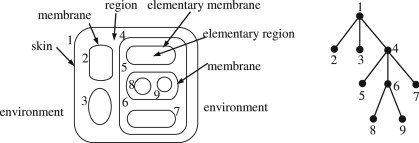
\includegraphics{img/membrane_structure.jpg}
  \caption{The membrane structure of a P system and its associated tree \cite{Zhang20101997AnalyzingRadarSignalsWithMembrane}}
  \label{fig:membrane_structure}
\end{figure}

% Membrane models

Recently, several computational models based on the membrane structure have been created.



% P systems

\subsubsection{P systems} % (fold)
\label{subs:p_systems}

\index{P systems} P systems (see \cite{Paun98}) were introduced in 1998 as a system with membrane structure that contains multisets of objects and rewriting rules that are executed in a maximally parallel manner. Since then, a huge amount of variants have been created with various computation powers. We have investigated the computational power and other attributes of several such variants. Additionally, we propose a new variants various notions of emptyness detection, where the rules can describe what will happen to an object that arrives to an empty membrane.

P systems with existing and newly proposed variants will be discussed in the chapter \ref{cha:p_systems}.

Aside from P systems, other models based on the membrane structure have been created such as the Calculus of Looping Sequences (CLS), which was inspired by P systems.

% subsubsection p_systems (end)


% CLS

\subsubsection{The Calculus of Looping Sequences} % (fold)
\label{subs:calculus_of_looping_sequences}

In the last few years many formalisms originally developed by computer scientists to model systems of interacting components have been applied to biology. Here, we can mention Petri nets (see section \ref{sec:petri_nets}). Others, such as P systems (see chapter \ref{cha:p_systems}), have been proposed as biologically inspired computational models and have been later applied to the description of biological systems.

Many of these models either offer only very low-level interaction primitives or they are specialized to the description of some particular kinds of phenomena such as membrane interactions or protein interactions making the model be not so flexible to allow describing easily new activities observed on membranes without extending the formalism to model such activities.

Barbuti in \cite{Barbuti07CLS} concluded that there is a need for a formalism having a simple notation, having the ability of describing biological systems at different levels of abstractions, having some notions of compositionality and being flexible enough to allow describing new kinds of phenomena as they are discovered, without being specialized to the description of a particular class of systems. The \index{Calculus of Looping Sequences} Calculus of Looping Sequences (CLS) was introduced in \cite{Barbuti07CLS}.

A CLS model consists of a term and a set of rewriting rules. The term is intended to represent the structure of the modeled system and the rewriting rules to represent the events that may cause the system to evolve.

The membrane structure in CLS is defined recursively, consisting of terms and sequences.

We start with defining the syntax of terms. We assume a possibly infinite alphabet $\Sigma$ of symbols.

\begin{definition}
  Terms $T$ and sequences $S$ of CLS are given by the following grammar:
  \begin{align*}
    T ::= S \bigpipe (S)^L\rfloor T \bigpipe T|T\\
    S ::= \eps \bigpipe a \bigpipe S\cdot S
  \end{align*}
  where $a\in \Sigma$ and $\eps$ represents the empty sequence. We denote with $\mathcal T$ the infinite set of terms and with $\mathcal S$ the infinite set of sequences.
\end{definition}

\begin{figure}
  \centering
  \begin{tikzpicture}[node distance=16mm,-triangle 45]
    \node(a){a};
    \node[right=12mm of a](f){f};
    \node[right= of f](g){g};
    \node[right=12mm of g](c){c};
    \node[below=10mm of f](d){d};
    \node[right= of d](e){e};
    \node[below right=16mm and 8mm of d.center](b){b};
    \node[below=10mm of b](description){A representation of the term $(a\cdot b\cdot c)^L\rfloor ((d\cdot e)^L | f\cdot g)$.};
    \draw (a) edge[bend right=60] (b);
    \draw (b) edge[bend right=60] (c);
    \draw (c) edge[bend right=60] (a);
    \draw (d) edge[bend right=60] (e);
    \draw (e) edge[bend right=60] (d);
    \draw (f) edge (g);
  \end{tikzpicture}
  \caption{Example CLS}
  \label{fig:example cls}
\end{figure}

In CLS we have a sequencing operator $\_\cdot\_$, a looping operator $(\_)^L$, a parallel composition operator $\_|\_$ and a containment operator $\_\rfloor\_$. Sequencing can be used to concatenate elements of the alphabet $\Sigma$. The empty sequence $\eps$ denotes the concatenation of zero symbols. A term can be either a sequence or a looping sequence (that is the application of the looping operator to a sequence) containing another term, or the parallel composition of two terms. By definition, looping and containment are always applied together, hence we can consider them as a single binary operator $(\_)^L\rfloor\_$ which applies to one sequence and one term.

\begin{example}
  In the Figure \ref{fig:example cls} we show an example of CLS and its visual representation. The same structure may be represented by syntactically different terms, e.g. $(b\cdot c\cdot a)^L\rfloor (f\cdot g | (e\cdot d)^L)$. We introduce a structural congruence relation to identify such terms.
\end{example}

\begin{definition}
  The structural congruence relations $\equiv_S$ and $\equiv_T$ are the least congruence relations on sequences and on terms, respectively, satisfying the following rules:
  \begin{itemize}
    \item $S_1\cdot(S_2\cdot S_3)\equiv_S (S_1\cdot S_2)\cdot S_3$
    \item $S\cdot\eps\equiv_S \eps\cdot S\equiv_S S$
    \item $S_1\equiv_S S_2$ implies $S_1\equiv_T S_2$ and $(S_1)^L\rfloor T\equiv_T (S_2)^L\rfloor T$
    \item $T_1|T_2\equiv_T T_2|T_1$
    \item $T_1|(T_2|T_3)\equiv_T (T_1|T_2)|T_3$
    \item $T|\eps\equiv_T T$
    \item $(\eps)^L\rfloor\eps\equiv_T\eps$
    \item $(S_1\cdot S_2)^L\rfloor T\equiv_T (S_2\cdot S_1)^L\rfloor T$
  \end{itemize}
\end{definition}

Note that the last rule does not introduce the commutativity of sequences, but only says that looping sequences can rotate.

What could look strange in CLS is the use of looping sequences for the description of membranes, as sequencing is not a commutative operation and this does not correspond to the usual fluid representation of membrane surface in which objects can move freely. What one would expect is to have a multiset or a parallel composition of objects on a membrane. For this reason, a variant called CLS+ was introduced in \cite{Milazzo07CLS}, in which the looping operator can be applied
to a parallel composition of sequences.

\begin{definition}
  Terms $T$, branes $B$ and sequences $S$ of CLS+ are given by the following grammar:
  \begin{align*}
    T ::= S \bigpipe (B)^L\rfloor T \bigpipe T|T\\
    B ::= S \bigpipe B|B\\
    S ::= \eps \bigpipe a \bigpipe S\cdot S
  \end{align*}
\end{definition}

The structural congruence relation of CLS+ is a trivial extension of the one of CLS. The only difference is that commutativity of branes replaces rotation of looping sequences. CLS+ models can be translated into CLS models, while preserving the semantics of the model \cite{Barbuti07CLS}. Milazzo in his PhD thesis \cite{Milazzo07CLS} includes also a simulation of a P system using CLS. The major difficulty was the simulation of the maximal parallel rule application.

% subsubsection calculus_of_looping_sequences (end)

% subsection membrane_systems (end)

% section biologically_inspired_computing_models (end)

% chapter natural_computing (end)

\chapter{Preliminaries} % (fold)
\label{cha:preliminaries}
This chapter is about some basic notions of computer science which will be used through the work. We start by defining formal languages and basic models (grammars, machines) that define language families and end by defining multiset languages.

\section{Formal languages} % (fold)
\label{sec:formal_languages}

Our study is based on the classical theory of formal languages. We will recall some definitions:

\begin{definition}
An {\bf alphabet} is a finite nonempty set of symbols.
\end{definition}

\begin{definition}
A {\bf string} over an alphabet is a finite sequence of symbols from alphabet.
\end{definition}

The length of the string $s$ is denoted by $|s|$. We denote by $V^*$ the set of all strings over an alphabet $V$. By $V^+$ = $V^* - \{\eps\}$ we denote the set of all nonempty strings over V.

\begin{definition}
A {\bf language} over the alphabet $V$ is any subset of $V^*$.
\end{definition}

\begin{definition}
A {\bf family of languages} is a set of languages.
\end{definition}


\section{Formal grammars} % (fold)
\label{sec:formal_grammars}

\begin{definition}
A {\bf formal grammar} is a tuple $G = (N,T,P,\sigma)$, where
\begin{itemize}
  \item $N, T$ are disjoint alphabets of non-terminal and terminal symbols,
  \item $\sigma\in N$ is the initial non-terminal,
  \item $P$ is a finite set of rewriting rules of the form $u\rightarrow v$, with $u\in (N\cup T)^*N(N\cup T)^*$ and $v\in (N\cup T)^*$.
\end{itemize}
\end{definition}

\begin{definition}
A {\bf rewriting step} in the grammar $G$ is a binary relation $\Rightarrow$ on $(N\cup T)^*$, where $x\Rightarrow y$ only if $\exists w_1, w_2\in (N\cup T)^+$ and a rule $u\rightarrow v \in P$ such that $x=w_1uw_2$ and $y=w_1vw_2$.
\end{definition}

\begin{definition}
Language defined by a grammar $G$ is a set $L(G)=\{w\in T^*|\sigma\Rightarrow w\}$.
\end{definition}

Languages that can be generated by a formal grammar are the recursively enumerable languages $RE$.

% section formal_languages (end)

% section formal_grammars (end)

\section{Chomsky hierarchy} % (fold)
\label{sec:chomsky_hierarchy}

In this section we introduce several well-known families of languages.

\begin{definition}
A {\bf regular grammar} is a formal grammar, where the rewriting rules are of the form $u\rightarrow v$, where $u\in N$ and $v\in T^*(N\cup \{\eps\})$.
\end{definition}

\begin{definition}
A {\bf regular language} is a language generated by a regular grammar. The family of regular languages is denoted $R$.
\end{definition}

\begin{definition}
A {\bf context-free grammar} is a formal grammar, where rewriting rules are of the form $u\rightarrow v$, where $u\in N$ and $v\in (N\cup T)^*$.
\end{definition}

\begin{definition}
A {\bf context-free language} is a language generated by a context-free grammar. The family of context-free languages is denoted $CF$.
\end{definition}

\begin{definition}
A {\bf context-sensitive grammar} is a formal grammar, where rewriting rules are of the form $u\rightarrow v$, where $u\in (N\cup T)^*N(N\cup T)^*$, $v\in (N\cup T)^*$ and $|u| < |v|$.
\end{definition}

\begin{definition}
A {\bf context-sensitive language} is a language generated by a context-sensitive grammar. The family of context-sensitive languages is denoted $CS$.
\end{definition}

These families of languages forms the Chomsky hierarchy by means of inclusions: $R \subset CF \subset CS \subset RE$.

% section chomsky_hierarchy (end)

\section{Matrix grammars} % (fold)
\label{sec:matrix_grammars}

\begin{definition}
A {\bf matrix grammar} is a tuple $G = (N,T,M,\sigma)$, where:
\begin{itemize}
  \item $N, T$ are disjoint alphabets of non-terminal and terminal symbols,
  \item $\sigma\in N$ is the initial non-terminal,
  \item $M$ is a finite set of matrices, which are sequences of context-free rules of the form $u\rightarrow v$, where $u\in N$ and $v\in (N\cup T)^*$.
\end{itemize}
\end{definition}

\begin{definition}
A {\bf rewriting step} $x\Rightarrow y$ holds only if there is a matrix $(u_1\rightarrow v_1, u_2\rightarrow v_2, \ldots, u_n\rightarrow v_n) \in M$ such that for each $1\leq i\leq n$ the following holds: $x_i = x_i^{\prime}u_ix_i^{\prime\prime}$ and $x_{i+1} = x_i^{\prime}v_ix_i^{\prime\prime}$, where $x_i, x_i^{\prime}, x_i^{\prime\prime} \in (N\cup T)^*$ and $x_1 = x$ and $x_{n+1} = y$.
\end{definition}

\begin{example}
Consider the matrix grammar $G=(\{\sigma, X,Y\}, \{ a,b,c\}, M, \sigma)$, where $M$ contains three matrices: $[S\rightarrow XY], [X\rightarrow aXb, Y\rightarrow cY], [X\rightarrow ab, Y\rightarrow c]$. There are only context-free rules, yet the grammar generate the context-sensitive language $\{a^nb^nc^n|n\geq 1\}$.
\end{example}

The family of matrix grammars is denoted $MAT$.

It is known that $CF \subset MAT \subset RE$. Interestingly, $MAT \cap {a}^* \subset R$ (see \cite{Besozzi:PhD:2004}).

% section matrix_grammars (end)

\section{Register machines} % (fold)
\label{sec:register_machines}

% We will use the notion of register machine as defined in our article

\begin{definition}
  A {\bf $n$-register machine} is a tuple $M = (n,P,i,h)$, where:
  \begin{itemize}
    \item $n$ is the number of registers,
    \item $P$ is a set of labeled instructions of the form $j : (op(r),k,l)$, where $op(r)$ is an operation on register $r$ of $M$, and $j$, $k$, $l$ are labels from the set $Lab(M)$ (which numbers the instructions in a one-to-one manner),
    \item $i$ is the initial label, and
    \item $h$ is the final label.
  \end{itemize}
\end{definition}

The machine is capable of the following instructions:
\begin{itemize}
\item $(add(r),k,l)$ : Add one to the contents of register $r$ and proceed to instruction $k$ or to instruction $l$; in the deterministic variants usually considered in the literature we demand $k = l$.
\item $(sub(r),k,l)$ : If register $r$ is not empty, then subtract one from its contents and go to instruction $k$, otherwise proceed to instruction $l$.
\item $halt$ : This instruction stops the machine. This additional instruction can only be assigned to the final label $h$.
\end{itemize}

A deterministic $m$-register machine can analyze an input $(n_1,\dots,n_m)\in N_0^m$ in registers 1 to $m$, which is recognized if the register machine finally stops by the halt instruction with all its registers being empty (this last requirement is not necessary). If the machine does not halt, the analysis was not successful.

% section register_machines (end)

\section{Lindenmayer systems} % (fold)
\label{sec:lindenmayer_systems}

In 1968, a Hungarian botanist and theoretical biologist Aristid Lindenmayer introduced \cite{Lindenmayer68} a new string rewriting algorithm named Lindenmayer systems (or L-systems for short). They are used by biologists and theoretical computer scientists to mathematically model growth processes of living organisms, especially plants. The difference with Chomsky grammars is that rewriting is parallel, not sequential.

The simplest version of L-systems assumes that the development of a cell is free of influence of other cells.
This type of L-systems is called $0L$ systems, where ``0'' stands for zero-sided communication between cells.

\begin{definition}
A $0L$ system is a triple $(\Sigma, P, \omega)$, where $\Sigma$ is an alphabet, $\omega$ is a word over $\Sigma$ and $P$ is a finite set of rewriting rules of the form $a\rightarrow x$, where $a\in\Sigma, x\in\Sigma^*$.
\end{definition}

It is assumed there is at least one rewriting rule for each letter of $\Sigma$. $0L$ system works in parallel way, so all the symbols are rewritten in each step.

\begin{example}
Consider a $0L$ system with alphabet $\Sigma = \{a,b\}$, initial word $\omega = a$ and rewriting rules $P = \{a\rightarrow b, b\rightarrow ab\}$.
Since in this system there is exactly one rule for every letter of the alphabet, the rewriting is thus deterministic and the generated words will be $\{a, b, ab, bab, abbab, \ldots \}$. 
\end{example}

$1L$ systems allows the rewriting rules to include context of size 1, so it allows for rules of type $yaz\rightarrow x$.

L-systems with tables ($T$) have several sets of rewriting rules instead of just one set. At one step of the rewriting process, rules belonging to the same set have to be applied. The biological motivation for introducing tables is that one may want different rules to take care of different environmental conditions (heat, light, etc.) or of different stages of development.

\begin{definition}
An extended ($E0L$) system is a pair $G_1 = (G, \Sigma_T)$, where $G = (\Sigma, P, \omega)$ is an $0L$ system, where $\Sigma_T \subseteq \Sigma$, referred to as the terminal alphabet. The language generated by $G_1$ is defined by $L(G_1) = L(G)\cap \Sigma_T^*$.
\end{definition}

Such languages are called $E0L$ languages. $E0L$ languages with tables are called $ET0L$ languages.

It is known that $CF \subset E0L \subset ET0L \subset CS$ (see section \ref{sec:chomsky_hierarchy} for definitions of $CF$ and $CS$).
% section lindenmayer_systems (end)

\section{Multisets} % (fold)
\label{sec:multisets}

\begin{definition}
A multiset over a set $X$ is a mapping $M: X\rightarrow \mathbb N$.
\end{definition}

We denote by $M(x), x\in X$ the multiplicity of $x$ in the multiset $M$.

\begin{definition}
The {\bf support} of a multiset $M$ is the set $supp(M)=\{x\in X|M(x)\geq 1\}$.
\end{definition}

It is the set of items with at least one occurrence.

\begin{definition}
A multiset is {\bf empty} when its support is empty.
\end{definition}

A multiset $M$ with finite support $X = \{x_1, x_2, \ldots, x_n\}$ can be represented by the string $x_1^{M(x_1)}x_2^{M(x_2)}\ldots x_n^{M(x_n)}$.
As elements of a multiset can also be strings, we separate them with the pipe symbol, e.g. $$element|element|other\_element$$.

\begin{definition}
Multiset inclusion. We say that multiset $M_1$ is included in multiset $M_2$ if $\forall x \in X: M_1(x)\leq M_2(x)$. We denote it by $M_1\subseteq M_2$.
\end{definition}

\begin{definition}
The {\bf union} of two multisets $M_1\cup M_2$ is a multiset where $\forall x \in X: (M_1\cup M_2)(x)=M_1(x)+M_2(x)$.
\end{definition}

\begin{definition}
The {\bf difference} of two multisets $M_1-M_2$ is a multiset where $\forall x \in X: (M_1-M_2)(x)=M_1(x)-M_2(x)$.
\end{definition}

\begin{definition}
Product of multiset $M$ with natural number $n\in \mathbb N$ is a multiset where $\forall x \in X: (n\cdot M)(x)=n\cdot M(x)$.  
\end{definition}

% section multisets (end)

\section{Semilinear sets} % (fold)
\label{sec:semilinear_sets}

\begin{definition}
  A {\bf linear set} $L(c,p_1,\ldots,p_r)$ is a subset $\{c+\sum\limits_{i=1}^r|k_i\in\mathbb N\}$ of $\mathbb N^n$, where $c,p_1,\ldots,p_r\in \mathbb N^n$.
\end{definition}

We call $c$ the constant and $p_1,\ldots,p_r$ the periods of the linear set.

\begin{example}
  For $n=1$ the linear set is a subset of $\mathbb N$. For $n=1$ and $r=1$ we get an arithmetic progression.
\end{example}

\begin{example}
  $L((0,0),(0,1),(1,0))$ contains all pairs with one zero element and one non-negative element: $$\{(0,0), (1,0), (2,0), \ldots, (x,0), \ldots, (0,1), (0,2), \ldots, (0,y), \ldots\}$$.
\end{example}

\begin{definition}
  A subset of $\mathbb N^n$ is called {\bf semilinear} if it is a finite union of linear sets.
\end{definition}

\subsection{Parikh's mapping} % (fold)
\label{sec:parikh_s_mapping}

In this subsection we show how semilinear sets and multisets relate to the formal language theory. We will start with several basic definitions.

The number of occurrences of a given symbol $a\in \Sigma$ in the string $w\in \Sigma^*$ is denoted by $|w|_a$.

\begin{definition}
$\Psi_\Sigma(w)=(|w|_{a_1},|w|_{a_2},\ldots,|w|_{a_n})$ is called a {\bf Parikh image of the string} $w\in \Sigma^*$, where $\Sigma=\{a_1,a_2,\ldots a_n\}$.
\end{definition}

When referring to the Parikh mapping for a language, this should be taken to mean the mapping applied to all the words on the language. This idea is expressed in the next definition. 

\begin{definition}
For a language $L\subseteq \Sigma^*$, $\Psi_\Sigma(L)=\{\Psi_\Sigma(w)|w\in L\}$ is the {\bf Parikh image of the language} $L$.
\end{definition}

\begin{definition}
If $FL$ is a family of languages, by $PsFL$ we denote the family of Parikh images of languages in $FL$, e.g. $PsCF, PsRE$.
\end{definition}

\begin{example}
Consider an alphabet $V=\{a,b\}$ and a language $L=\{a, ab, ba\}$.
$\Psi_\Sigma(L)=\{(1,0), (1,1)\}$. Notice that Parikh image of $L$ has only 2 element while $L$ has 3 elements.
\end{example}

\begin{example}
  Consider the context-free grammar $G = (N,T,P,\sigma)$, where $N=\{A,B\}$, $T=\{a,b\}$ and with rules $P=\{\sigma\rightarrow A\sigma B|B\sigma A|ab, A\rightarrow a, B\rightarrow b\}$.

  This means that the language generated by $G$ contains strings where $a$s and $b$s can occur intermixed. But, as is clear from the language definition, the same number of $a$s and $b$s will always be present. Moreover, there will always be at least one of each letters.

  Consider the words $w_1 = aaaabbbb \in L(G)$ and $w_2 = babababa \in L(G)$. Both of these words have the same Parikh image: $\Psi_\Sigma(w_i) = (4,4)$. It is interesting to note that most information embedded in a word generated with a context-free grammar is thrown away by the Parikh mapping.
\end{example}

This loss of information is expressed in the Parikh's theorem \cite{Parikh66}, stating that the Parikh image of a context-free language is semilinear. The biggest implication of the theorem though, is that it shows that if the order of the symbols is ignored, then it is impossible to distinguish between a regular set and a context-free language \cite{Kozen97Automata}.

Another interesting result appeared in \cite{Ito69Semilinear} that every semilinear set is a finite union of disjoint linear sets.

% subsection parikh_s_mapping (end)

% section semilinear_sets (end)

\section{Petri nets} % (fold)
\label{sec:petri_nets}

Petri nets \cite{Petri62,Yen06PetriNets} were introduced by Carl Adam Petri in 1962 in his PhD thesis. A Petri net is a graphical and mathematical tool for the modeling of concurrent processes and analysis of system behavior. A Petri net is usually drawn as a directed bipartite graph with two kind of nodes. Places are represented by circles within which each small black dot denotes a token. Transitions are represented by bars. Each edge is either from a place to a transition or vice versa.

\begin{definition}
  A {\bf Petri net} is a tuple $(P, T, \varphi)$, where:
  \begin{itemize}
    \item $P$ is a finite set of places,
    \item $T$ is a finite set of transitions,
    \item $\varphi: (P\times T)\cup(T\times P)\rightarrow \mathbb N$ is a flow function.
  \end{itemize}
\end{definition}

The edges of the bipartite graph are annotated by either $\varphi(p,t)$ or $\varphi(t,p)$, where $p\in P$ and $t\in T$ are two endpoints of the arc. If $\varphi(p,t)=1$ or $\varphi(t,p)=1$, we usually omit the label.

\begin{definition}
  A {\bf marking} is a mapping $\mu: P\rightarrow \mathbb N$.
\end{definition}

The mapping $\mu$ assigns certain number of tokens to each place of the net.

\begin{definition}
  A marking $\mu_1$ {\bf covers} marking $\mu_2$, when $\forall p\in P: \mu_1(p)\geq\mu_2(p)$ - in each place there is no less tokens in $\mu_1$ than in $\mu_2$. We denote it by $\mu_1\geq\mu_2$.
\end{definition} 

\begin{definition}
  A transition $t\in T$ is {\bf enabled} at a marking $\mu$ iff $\forall p\in P, \varphi(p,t)\leq\mu(p)$.
\end{definition}

If a transition $t$ is enabled, it may fire by removing $\varphi(p,t)$ tokens from each input place $p$ and putting $\varphi(t,p^\prime)$ tokens in each output place $p^\prime$. We then write $\mu\xrightarrow{t} \mu^\prime$, where $\forall p\in P: \mu^\prime(p) = \mu(p)-\varphi(p,t)+\varphi(t,p)$.

\begin{example}
  In the Figure \ref{fig:example petri net} the Petri net has four places and two transitions. At the current marking the transition $t_1$ is enabled and the transition $t_2$ is not enabled. Firing the transition $t_1$ takes one token from the place $p_1$ and produces one token to places $p_2, p_3$ and $p_4$. In the resulting marking both transitions $t_1$ and $t_2$ are enabled.
\end{example}

\begin{definition}
  A {\bf marked Petri net} is a tuple $(P,T,\varphi,\mu_0)$, where $(P,T,\varphi)$ is a Petri net and $\mu_0$ is called the initial marking.
\end{definition}

\begin{definition}
  A sequence of transitions $\sigma = t_1\ldots t_n$ is a {\bf firing sequence} from $\mu_0$ iff $\mu_0\xrightarrow{t_1}\mu_1\xrightarrow{t_2}\ldots\xrightarrow{t_n}\mu_n$ for some markings $\mu_1,\ldots,\mu_n$. We also write $\mu_0\xrightarrow{\sigma}\mu_n$.
\end{definition}

We write $\mu_0\xrightarrow{\sigma}$ to denote that $\sigma$ is enabled and can be fired from $\mu_0$, i.e., $\mu_0\xrightarrow{\sigma}$ iff there exists a marking $\mu$ such that $\mu_0\xrightarrow{\sigma}\mu$.
The notation $\mu_0\xrightarrow{*}\mu$ is used to denote the existence of a firing sequence $\sigma$ such that $\mu_0\xrightarrow{\sigma}\mu$.

\begin{definition}
  A marking $\mu$ is reachable for a marked Petri net $\mathcal P = (P,T,\varphi,\mu_0)$ iff $\mu_0\xrightarrow{*}\mu$.
\end{definition}

\begin{definition}
  Let $\mathcal P = (P,T,\varphi,\mu_0)$ be a marked Petri net. The {\bf reachability set} of $\mathcal P$ is $R(\mathcal(P)) = \{\mu|\mu_0\xrightarrow{*}\mu\}$.
\end{definition}

A notion of reachability graph is helpful for analyzing the behavior of a Petri net as a tool for visualisation of the structure of the reachability set.

\begin{definition}
  Let $\mathcal P = (P,T,\varphi,\mu_0)$ be a marked Petri net. The {\bf reachability graph} of $\mathcal P$ is a labelled graph whose nodes are the reachable markings and edge from $\mu_1$ to $\mu_2$ is labeled with a transition $t\in T$ iff $\mu_1\xrightarrow{t}\mu_2$.
\end{definition}

\begin{figure}
  \centering
  \begin{minipage}{.4\textwidth}
    \begin{tikzpicture}
      \tikzstyle{transition}=[rectangle,thick,fill=black,minimum height=8mm]
      \node [place,tokens=3,label=above:$p_1$] (p1) {};
      \node [transition,label=above:$t_1$] (t1) [right of=p1] {}
        edge [pre] (p1);
      \node [place,tokens=0,label=right:$p_3$] (p3) [right of=t1] {}
        edge [pre] (t1);
      \node [place,tokens=0,label=right:$p_2$] (p2) [above of=p3] {}
        edge [pre] (t1);
      \node [place,tokens=0,label=right:$p_4$] (p4) [below of=p3] {}
        edge [pre] (t1);
      \node [transition,label=below:$t_2$] (t2) [below of=t1] {}
        edge [pre] (p4)
        edge [post] (p1);
    \end{tikzpicture}
    \captionof{figure}{An example Petri net}
    \label{fig:example petri net}
  \end{minipage}
  \hspace{.08\textwidth}
  \begin{minipage}{.4\textwidth}
    \begin{tikzpicture}[node distance=8mm,-triangle 45]
      \tikzstyle{every node} = [rectangle,draw]
      \tikzstyle{label} = [draw=none]
      \node (1) {3,0,0,0};
      \node [below= of 1] (2) {2,1,1,1};
      \node [below= of 2] (3) {1,2,2,2};
      \node [below= of 3] (4) {0,3,3,3};
      \node [right= of 2] (5) {3,1,1,0};
      \node [below= of 5] (6) {2,2,2,1};
      \node [below= of 6] (7) {1,3,3,2};
      \node [below= of 7] (8) {1,4,4,3};
      \node [draw=none,right= of 6] (9) {$\ldots$};
      \node [draw=none,right= of 7] (10) {$\ldots$};
      \node [draw=none,right= of 8] (11) {$\ldots$};
      \draw (1) edge node [label,right] {$t_1$} (2);
      \draw (2) edge node [label,right] {$t_1$} (3);
      \draw (3) edge node [label,right] {$t_1$} (4);
      \draw (2) edge node [label,above] {$t_2$} (5);
      \draw (3) edge node [label,above] {$t_2$} (6);
      \draw (4) edge node [label,above] {$t_2$} (7);
      \draw (5) edge node [label,right] {$t_1$} (6);
      \draw (6) edge node [label,right] {$t_1$} (7);
      \draw (7) edge node [label,right] {$t_1$} (8);
      \draw (6) edge node [label,above] {$t_2$} (9);
      \draw (7) edge node [label,above] {$t_2$} (10);
      \draw (8) edge node [label,above] {$t_2$} (11);
    \end{tikzpicture}
    \captionof{figure}{An example reachability graph}
    \label{fig:example reachability graph}
  \end{minipage}
\end{figure}

\begin{example}
  Consider a Petri net $\mathcal P$ from the Figure \ref{fig:example petri net}. Its reachability graph is in the Figure \ref{fig:example reachability graph}. $\mathcal P$ is not bounded because by alternately firing transitions $t_1$ and $t_2$ we can reach infinitely many different markings. We can also easily see that it is live, because in every marking for every transition $t\in\{t_1, t_2\}$ there is a firing sequence ending with $t$.
\end{example}

In spite of its simplicity, the applicability of the technique of reachability graph analysis is rather limited in the sense that it suffers from the state explosion phenomenon as the sizes of the reachability sets grow beyond any primitive recursive function in the worst case \cite{Yen06PetriNets}.

Coverability graph analysis offers an alternative to the techinque of reachability graph analysis by abstracting out certain details to make the graph finite. To understand the intuition behind coverability graphs, consider the Figure \ref{fig:example reachability graph} which shows a part of the reachability graph of the Petri net in the Figure \ref{fig:example petri net}. Consider the path $(3,0,0,0)\xrightarrow{t_1}(2,1,1,1)\xrightarrow{t_2}(3,1,1,0)$ along which the places $p_2$ and $p_3$ both gain an extra token in the end, i.e. $(3,0,0,0) > (3,1,1,0)$. Clearly they can be made to contain arbitrary large number of tokens by repeating the firing sequence $t_1t_2$ for a sufficient number of times, as $(3,0,0,0)\xrightarrow{t_1t_2}(3,1,1,0)\xrightarrow{t_1t_2}(3,2,2,0)\xrightarrow{t_1t_2}\ldots\xrightarrow{t_1t_2}(3,n,n,0)$, for arbitrary $n$. In order to capture the notion of a place being unbounded, we short-circuit the above infinite sequence of computation as $(3,0,0,0)\xrightarrow{t_1}(2,1,1,1)\xrightarrow{t_2}(3,\omega,\omega,0)$, where $\omega$ is a symbol denoting something being arbitrarily large. As it turns out, the coverability graph of a Petri net is always finite \cite{Karp69ParallelProgramSchemata}. The corresponding coverability graph of the example Petri net in the Figure \ref{fig:example petri net} is in the Figure \ref{fig:example coverability graph}. The algorithm for generating the coverability graph of a Petri net is shown \vpageref[above]{alg:coverability_graph}.

\begin{figure}
  \centering
  \begin{tikzpicture}[node distance=8mm,-triangle 45]
    \tikzstyle{every node} = [rectangle,draw]
    \tikzstyle{label} = [draw=none]
    \node (1) {3,0,0,0};
    \node [below= of 1] (2) {2,1,1,1};
    \node [below= of 2] (3) {1,2,2,2};
    \node [below= of 3] (4) {0,3,3,3};
    \node [right= of 2] (5) {$3,\omega,\omega,0$};
    \node [below= of 5] (6) {$2,\omega,\omega,1$};
    \node [below= of 6] (7) {$1,\omega,\omega,2$};
    \node [below= of 7] (8) {$1,\omega,\omega,3$};
    \draw (1) edge node [label,right] {$t_1$} (2);
    \draw (2) edge node [label,right] {$t_1$} (3);
    \draw (3) edge node [label,right] {$t_1$} (4);
    \draw (2) edge node [label,above] {$t_2$} (5);
    \draw (3) edge node [label,above] {$t_2$} (6);
    \draw (4) edge node [label,above] {$t_2$} (7);
    \draw (5) edge [bend right=30] node [label,left] {$t_1$} (6);
    \draw (6) edge [bend right=30] node [label,left] {$t_1$} (7);
    \draw (7) edge [bend right=30] node [label,left] {$t_1$} (8);
    \draw (6) edge [bend right=30] node [label,right] {$t_2$} (5);
    \draw (7) edge [bend right=30] node [label,right] {$t_2$} (6);
    \draw (8) edge [bend right=30] node [label,right] {$t_2$} (7);
  \end{tikzpicture}
  \caption{An example coverability graph}
  \label{fig:example coverability graph}
\end{figure}

\begin{algorithm}
  \caption{Coverability graph algorithm}\label{alg:coverability_graph}
  \begin{algorithmic}[1]
    \Procedure{CoverabilityGraph}{marked Petri net $\mathcal P = (P, T, \varphi, \mu_0)$}
      \State $\text{create a node $\mu_{init}$ such that $\mu_{init} = \mu_0$ and mark it as `new'}$
      \While{$\text{there is a `new' node $\mu$}$}
        \For{$\text{each transition $t$ enabled at $\mu$}$}
          \If{$\text{there is a node $\mu^\prime=\mu+\Delta t$}$}
            \State $\text{add an edge $\mu\xrightarrow{t}\mu^\prime$}$
          \ElsIf{$\text{there is a path $\mu_{init}\xrightarrow{*}\mu^{\prime\prime}\xrightarrow{*}\mu$ such that $\mu^{\prime\prime}<\mu+\Delta t$}$}
            \State $\text{add a `new' node $x$ with}$
            \State \hspace{\algorithmicindent}$\text{$x(p)=\omega$ if $\mu^{\prime\prime}(p)<(\mu+\Delta t)(p)$}$
            \State \hspace{\algorithmicindent}$\text{$x(p)=\mu^{\prime\prime}(p)$ otherwise}$
            \State $\text{add an edge $\mu\xrightarrow{t}x$}$
          \Else
            \State $\text{add a `new' node $x$ with $x=\mu+\Delta t$ and an edge $\mu\xrightarrow{t}x$}$
          \EndIf
        \EndFor
        \State $\text{mark $\mu$ with `old'}$
      \EndWhile
    \EndProcedure
  \end{algorithmic}
\end{algorithm}

\subsection{Analysis of behavioral properties} % (fold)
\label{sub:analysis_of_behavioral_properties}

Analysis of several behavioral properties is studied and following decidability problems are of special importance:

\subsubsection{The boundedness problem} % (fold)
\label{ssub:the_boundedness_problem}
  The boundedness problem is, given a marked Petri net $\mathcal P$, deciding whether $|R(\mathcal P)|$ is finite. This problem was first considered by Karp and Miller \cite{Karp69ParallelProgramSchemata}, where it was shown to be decidable using the technique of coverability graph analysis. A Petri net is unbounded iff an $\omega$ occurs in the corresponding coverability graph. The algorithm presented there was basically an unbounded search and consequently no complexity analysis was shown. Subsequently, a lower bound of $O(2^{cm})$ space was shown by Lipton in \cite{Lipton76Reachability}, where $m$ is the number of places in the Petri net and $c$ is a constant. Finally, an upper bound of $O(2^{cn\log{n}})$ space was given by Rackoff in \cite{Rackoff78Reachability}. Here, however, $n$ represents the size or number of bits in the problem instance and $c$ is a constant.
% subsubsection the_boundedness_problem (end)

\subsubsection{The covering problem} % (fold)
\label{ssub:the_covering_problem}
  The covering problem is, given a marked Petri net $\mathcal P$ and a marking $\mu$, deciding whether there exists $\mu^\prime\in R(\mathcal P)$ such that $\mu^\prime\geq\mu$. The complexity (both upper and lower bounds) of the covering problem can be derived along a similar line of that of the boundedness problem \cite{Rackoff78Reachability}.
% subsubsection the_covering_problem (end)

\subsubsection{The reachability problem} % (fold)
\label{ssub:the_reachability_problem}
  The reachability problem is, given a marked Petri net $\mathcal P$ and a marking $\mu$, deciding whether $\mu\in R(\mathcal P)$. This problem has attracted the most attention in the Petri net community. One reason is that the problem has many real-world applications; furthermore, it is the key to the solutions of several other Petri net problems. Before the decidability question of the reachability problem for general Petri nets was proven by Mayr in 1981 \cite{Mayr81PetriNetReachability}, a number of attempts had been made to investigate the problem for restricted classes of Petri nets, in hope of gaining more insights and developing new tools in order to conquer the general Petri net reachability problem. It should be noted that the technique of the coverability graph analysis does not answer the reachability problem as $\omega$ abstracts out the exact number of tokens that a place can accumulate, should the place be potentially unbounded.
% subsubsection the_reachability_problem (end)

\subsubsection{The containment problem} % (fold)
\label{ssub:the_containment_problem}
  The containment problem is, given two marked Petri nets $\mathcal P_1$ and $\mathcal P_2$, deciding whether $R(\mathcal P_1)\subseteq R(\mathcal P_2)$. In the late 1960's, Rabin first showed the containment problem for Petri nets to be undecidable. Even though the original work of Rabin have never been published, a new proof based on Hilbert's Tenth Problem \cite{Davis73Hilbert} was presented at MIT in 1972 \cite{Baker73PetriNetContainment}.
% subsubsection the_containment_problem (end)

\subsubsection{The equivalence problem} % (fold)
\label{ssub:the_equivalence_problem}
  The equivalence problem: given two marked Petri nets $\mathcal P_1$ and $\mathcal P_2$, deciding whether $R(\mathcal P_1) = R(\mathcal P_2)$. In 1975, Hack \cite{Hack1976PetriNetEquivalence} extended Rabin's result of the containment problem by showing the equivalence problem to be undecidable as well. The proof was also based on Hilbert's Tenth Problem.
% subsubsection the_equivalence_problem (end)

\subsubsection{The liveness problem} % (fold)
\label{ssub:the_liveness_problem}
  The liveness problem: given a marked Petri net $\mathcal P$, deciding whether for every $t\in T, \mu\in R(\mathcal P)$ there exists a sequence of transitions $\sigma$ such that $\mu\xrightarrow{\sigma t}$, i.e. $t$ is enabled after firing $\sigma$ from $\mu$. In \cite{Hack74PetriNetLiveness}, several variants of the reachability problem were shown to be recursively equivalent. Among them is the single-place zero reachability problem, i.e. the problem of determining whether a marking with no tokens in a designated place can be reached. Hack also showed the single-place zero reachability problem to be recursively equivalent to the liveness problem, which is then as well decidable.
% subsubsection the_liveness_problem (end)

% subsection analysis_of_behavioral_properties (end)

% section petri_nets (end)

\section{Vector addition systems} % (fold)
\label{sec:vector_addition_systems}

Vector addition systems were introduced by Karp and Miller \cite{Karp69ParallelProgramSchemata}, and were later shown by Hack \cite{Hack74PetriVAS} to be equivalent to Petri nets.

\begin{definition}
  A {\bf vector addition system} (VAS) is a pair $G = (x, W)$, where $x\in \mathbb N^n$ is an initial vector and $W\subseteq \mathbb Z^n$ is a finite set of vectors, where $n>0$ is called the dimension of VAS.
\end{definition}

The initial vector is seen as the initial values of multiple counters and the vectors in $W$ are seen as actions that update the counters. These counters may never drop below zero. 

\begin{definition}
  The {\bf reachability set} of the VAS $G = (x,W)$ is the set \linebreak $R(G) = \{z | \exists v_1,\ldots,v_j\in W: z=x+v_1+\ldots+v_j \wedge \forall 1\leq i\leq j: x+v_1+\ldots+v_i\geq 0\}$.
\end{definition}

\begin{definition}
  A {\bf vector addition system with states} (VASS) is a tuple $G = (x, W, Q, T, p_0)$, where:
  \begin{itemize}
    \item $(x, W)$ is a vector addition system,
    \item $Q$ is a finite set of states,
    \item $T$ is a finite set of transitions of the form $p\rightarrow(q,v)$, where $v\in W$ and $p,q\in Q$ are states,
    \item $p_0\in Q$ is the starting state.
  \end{itemize}
\end{definition}

The transition $p\rightarrow(q,v)$ can be applied at vector $y$ in state $p$ and yields the vector $y+v$ in state $q$, provided that $y+v\geq 0$.

\begin{example}
  For the Petri net in the Figure \ref{fig:example petri net}, the corresponding VAS $(x,W)$ is:
  \begin{itemize}
    \item $x=(3,0,0,0)$,
    \item $W=\{(-1,1,1,1),(1,0,0,-1)\}$.
  \end{itemize}
\end{example}

It is known \cite{Hack74PetriVAS} that Petri nets, VAS and VASS are computationally equivalent.

% section vector_addition_systems (end)

\section{Büchi automaton} % (fold)
\label{sec:buchi_automaton}

% section buchi_automaton (end)

\section{Calculi of looping sequences} % (fold)
\label{sec:calculi_of_looping_sequences}

% section calculi_of_looping_sequences (end)

\section{Graph theory} % (fold)
\label{sec:graph_theory}

\begin{definition}
  A {\bf graph} is a pair $G = (V,E)$ of sets such that $E\subseteq V\times V$ and $V\cap E = \emptyset$. The elements of $V$ are the vertices (or nodes) of the graph $G$, the elements of $E$ are its edges.
\end{definition}

The vertex set of a graph $G$ is denoted by $V(G)$, its edge set as $E(G)$.

\begin{definition}
  The {\bf order of the graph} $G$ is the number of its vertices, denoted by $|G|$. Graphs are (in)finite iff their order is (in)finite.
\end{definition}

\begin{definition}
  A vertex $v\in V$ is {\bf incident} with an edge $e\in E$ iff $v\in e$, i.e. either $e=(v,y)$, where $y\in V$ or $e=(x,v)$, where $x\in V$.
\end{definition}

\begin{definition}
  Two vertices $x,y\in V(G)$ are {\bf adjacent} iff $(x,y)\in E(G)$.
\end{definition}

\begin{definition}
  A {\bf path} is a non-empty graph $P=(V,E)$, where $V=\{x_0, x_1, \ldots, x_k\}$ and $E=\{(x_i,x_{i+1})|0\leq i < k\}$ and the $x_i$ are all distinct.
\end{definition}

\begin{definition}
  If $P=(V,E)$ is a path where $V=\{x_0, x_1, \ldots, x_k\}$ and $|V|\geq 3$, then the graph $C = (V,E\cup\{(x_k,x_0)\})$ is called a {\bf cycle}. 
\end{definition}

\begin{definition}
  A graph $G=(V,E)$ is a {\bf subgraph} of a graph $G^\prime = (V^\prime, E^\prime)$ iff $V\subseteq V^\prime$ and $E\subseteq E^\prime$. We denote it by $G\subseteq G^\prime$ and also say that $G^\prime$ contains $G$.
\end{definition}

\begin{definition}
  A non-empty graph $G$ is called {\bf connected} iff any two of its vertices are linked by a path in $G$.
\end{definition}

\begin{definition}
  A graph not containing any cycle is called a {\bf forest}.
\end{definition}

\begin{definition}
  A connected forest is called a {\bf tree}.
\end{definition}

Sometimes it is convenient to consider one vertex of a tree as special. Such a vertex is then called the root of this tree.

\begin{definition}
  A tree $T$ with a fixed root is called a {\bf rooted tree}. The root node of $T$ is denoted by $r_T$.
\end{definition}

\begin{definition}
  Let $d$ be a node of a non-root tree $T$, i.e. $d\in V(T)\setminus \{r_T\}$. As $T$ is a tree, there is a unique path from $d$ to $r_T$ \cite{Diestel97Graphs}. The node adjacent to $d$ on that path is also unique and is called a {\bf parent node} of $d$ and is denoted by $parent_T(d)$.
\end{definition}

\begin{definition}
  Let $T_1, T_2$ be two rooted trees. A bijection $f: V(T_1)\rightarrow V(T_2)$ is an {\bf isomorphism} iff $\forall x,y\in V(T): (x,y)\in E(T_1)\Leftrightarrow (f(x), f(y))\in E(T_2)$.
\end{definition}

Rooted trees $T_1$ and $T_2$ are called isomorphic if there exists an isomorphism on their nodes.

% section graph_theory (end)

\section{Bisimulations} % (fold)
\label{sec:bisimulations}
\begin{definition}
  A {\bf state transition system} is a pair $(S, \rightarrow)$, where $S$ is a set of states and $\rightarrow\subseteq S\times S$ is a binary transition relation over $S$.
\end{definition}
  If $p,q\in S$, then $(p,q)\in \rightarrow$ is usually written as $p\rightarrow q$. This represents the fact that there is a transition from state $p$ to state $q$.

\begin{definition}
  A {\bf labelled state transition system} (LTS) is a tuple $(S, A, \rightarrow)$, where $S$ is a set of states, $A$ is a set of labels and $\rightarrow\subseteq S\times A\times S$ is a ternary transition relation.
\end{definition}
  If $p,q\in S$ and $a\in A$, then $(p,a,q)\in \rightarrow$ is usually written as $p\xrightarrow{a} q$. This represents the fact that there is a transition from state $p$ to state $q$ with a label $a$.

\begin{definition}
  Let $(S_1, A, \rightarrow)$ and $(S_2, A, \rightarrow)$ be two labelled transition systems.
  A {\bf simulation} is a binary relation $R\subseteq S_1\times S_2$ such that if $(s_1,s_2)\in R$ then for each $s_1\xrightarrow{a} t_1$ there is some $s_2\xrightarrow{a} t_2$ such that $(t_1, t_2)\in R$.
\end{definition}

\begin{definition}
  Let $(S_1, A, \rightarrow)$ and $(S_2, A, \rightarrow)$ be two labelled transition systems.
  A {\bf bisimulation} is a binary relation $R\subseteq S_1\times S_2$ such that if $(s_1,s_2)\in R$ then:
  \begin{enumerate}
    \item for each $s_1\xrightarrow{a} t_1$ there is some $s_2\xrightarrow{a} t_2$ such that $(t_1, t_2)\in R$,
    \item for each $s_2\xrightarrow{a} t_2$ there is some $s_1\xrightarrow{a} t_1$ such that $(t_1, t_2)\in R$.
  \end{enumerate}
\end{definition}
% section bisimulations (end)

% chapter preliminaries (end)

\chapter{P systems} % (fold)
\label{cha:p_systems}
\import{p-systems/}{main}

% chapter p_systems (end)

\chapter{On the edge of universality of sequential P systems} % (fold)
\label{cha:on_the_edge_of_universality_of_sequential_p_systems}

\import{edge/}{main}

% chapter on_the_edge_of_universality_of_sequential_p_systems (end)

\chapter{Generating membrane structures} % (fold)
\label{cha:generating_membrane_structures}
CLS, CLS+, CLS++, CLS-
% chapter generating_membrane_structures (end)

\chapter{Maximal parallel P systems with context-free rules} % (fold)
\label{cha:maximal_parallel_p_systems_with_context_free_rules}
Notes about how inhibitors help, how determinism may help, how allowing only rules $a|a\rightarrow \_$ may help, how inhibiting other rules may help.
% chapter maximal_parallel_p_systems_with_context_free_rules (end)

\chapter*{Conclusions}
\addcontentsline{toc}{chapter}{Conclusions}
We have studied several variants of sequential P systems in order to obtain universality without using maximal parallelism. A variant with rewriting rules that can use inhibitors was shown to be universal in both generating and accepting case. The generating model is able to simulate maximal parallel P system and the accepting model can simulate a register machine.

In addition, we have defined a new notion of vacuum, which is immediately created in the region that becomes empty. A new P system variant was introduced, which allowed the vacuum to be used on the left side of P system rewriting rules. The accepting case of this variant was shown to be universal by direct implementation of a register machine.

A lot of other variants deserve to be combined with the vacuum, so we suggest to research them more
thoroughly(non-cooperative rules, rules with priorities, decaying objects, deterministic steps, . . . ).
\backmatter

% \begin{thebibliography}{1}
\bibliography{diz}
% \end{thebibliography}

\appendix

\chapter{Štatistiky}
Tu budú štatistiky.

\printindex

\end{document}
